\documentclass[border=6pt]{standalone}
\usepackage{tikz}
\usetikzlibrary{arrows.meta,positioning,calc,shapes.geometric,fit,backgrounds,patterns,matrix,decorations.pathreplacing}
\begin{document}
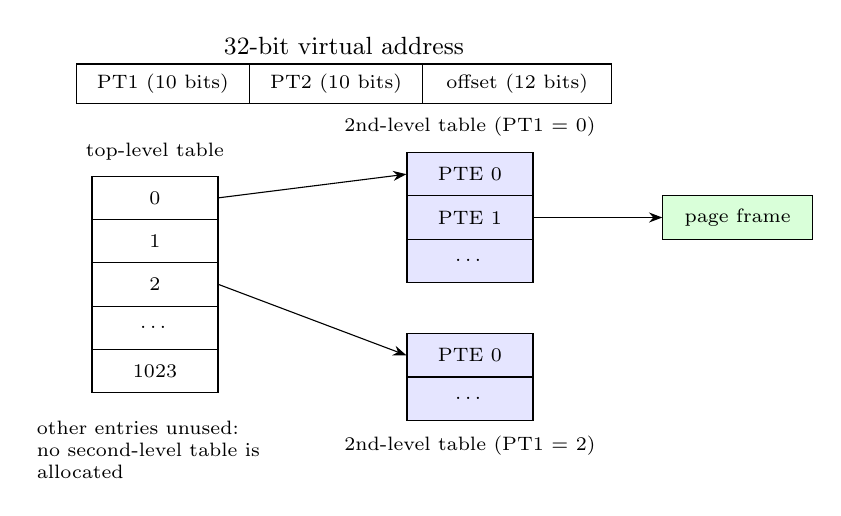
\begin{tikzpicture}[>=Stealth,font=\small]
\tikzstyle{c}=[draw,minimum height=0.55cm,minimum width=1.6cm,font=\scriptsize]
\draw (-1,2.4) rectangle node[font=\scriptsize]{PT1 (10 bits)} (1.2,2.9);
\draw (1.2,2.4) rectangle node[font=\scriptsize]{PT2 (10 bits)} (3.4,2.9);
\draw (3.4,2.4) rectangle node[font=\scriptsize]{offset (12 bits)} (5.8,2.9);
\node[above,font=\small] at (2.4,2.9) {32-bit virtual address};
\node[c] (t0) at (0,1.2) {0};\node[c] (t1) at (0,0.65) {1};\node[c] (t2) at (0,0.1) {2};\node[c] (t3) at (0,-0.45) {\ldots};\node[c] (t4) at (0,-1.0) {1023};
\node[font=\scriptsize,above=2pt of t0] {top-level table};
\node[c,fill=blue!10] (a0) at (4,1.5) {PTE 0}; \node[c,fill=blue!10] (a1) at (4,0.95) {PTE 1}; \node[c,fill=blue!10] (a2) at (4,0.4) {\ldots};
\node[font=\scriptsize,above=2pt of a0] {2nd-level table (PT1 = 0)};
\node[c,fill=blue!10] (b0) at (4,-0.8) {PTE 0}; \node[c,fill=blue!10] (b1) at (4,-1.35) {\ldots};
\node[font=\scriptsize,below=2pt of b1] {2nd-level table (PT1 = 2)};
\draw[->] (t0.east) -- (a0.west); \draw[->] (t2.east) -- (b0.west);
\node[c,fill=green!15,minimum width=1.9cm] (f) at (7.4,0.95) {page frame}; \draw[->] (a1.east) -- (f.west);
\node[font=\scriptsize,text width=3cm,align=left] at (0,-2.0) {other entries unused: no second-level table is allocated};
\end{tikzpicture}
\end{document}
